\documentclass[10pt,twocolumn,letterpaper]{article}
\makeatletter
\let\numberlines@hook\relax
\makeatother
\usepackage{cvpr}
\usepackage{times}
\usepackage{epsfig}
\usepackage{graphicx}
\usepackage{amsmath}
\usepackage{amssymb}
\usepackage{booktabs}
\usepackage[colorlinks,linkcolor=red,anchorcolor=blue,citecolor=green]{hyperref}
% Include other packages here, before hyperref.

% If you comment hyperref and then uncomment it, you should delete
% egpaper.aux before re-running latex.  (Or just hit 'q' on the first latex
% run, let it finish, and you should be clear).
\usepackage[breaklinks=true,bookmarks=false]{hyperref}

\cvprfinalcopy % *** Uncomment this line for the final submission

\def\cvprPaperID{****} % *** Enter the CVPR Paper ID here
\def\httilde{\mbox{\tt\raisebox{-.5ex}{\symbol{126}}}}

% Pages are numbered in submission mode, and unnumbered in camera-ready
%\ifcvprfinal\pagestyle{empty}\fi
\begin{document}
\title{CS 5787:  Deep Learning \\ Controllable Text-Image Generation with \\ Enhanced Text Encoder and Edge Loss}

\author{Xiaoyu Liang\\
(xl778)\\
% For a paper whose authors are all at the same institution,
% omit the following lines up until the closing ``}''.
% Additional authors and addresses can be added with ``\and'',
% just like the second author.
% To save space, use either the email address or home page, not both
\and
Zeyu Wang\\
(zw597)
\and
Cheng Wang\\
(cw859)
\and
Zhenglun Chen\\
(zc447)
}

\maketitle
%\thispagestyle{empty}

%%%%%%%%% ABSTRACT
\begin{abstract}
    Text-to-image generation through generative adversarial networks (GANs) has become a popular research topic in recent years in the fields of natural language processing and high-quality image synthesizing. Many text-to-image GAN algorithms have been proposed to generate realistic images that align the text query to a large extent, and most of them are based on learning latent word features which produces realistic characteristics though, but usually doesn’t capture the shape of the described item, generating images that contain out-of-shape items. In this paper, we remodeled an existing controllable text-to-image GAN  \cite{li2019controllable} by 1) modifying the encoders and 2) adding more kinds of losses as an attempt to improve model performance. Experiments on benchmark datasets demonstrate that our method outperforms existing state of the art based on the results retrieved from the 15th epoch, and is able to effectively manipulate synthetic images using natural language descriptions.
%   The ABSTRACT is to be in fully-justified italicized text, at the top
%   of the left-hand column, below the author and affiliation
%   information. Use the word ``Abstract'' as the title, in 12-point
%   Times, boldface type, centered relative to the column, initially
%   capitalized. The abstract is to be in 10-point, single-spaced type.
%   Leave two blank lines after the Abstract, then begin the main text.
%   Look at previous CVPR abstracts to get a feel for style and length.
\end{abstract}

%%%%%%%%% BODY TEXT
\section{Introduction}
\\\\
\noindent While text-to-image generators are widely applied in synthesizing images that match text description, big improvements were always achieved when the text/image encoding techniques were boosted. In the early days, most studies focused mainly on the adjustments to the image generation network, while generally regraded texts at sentence level instead of word level. As a result, those embedding outputs were relatively coarse since they lost many details of text information.
\\\\
Later, in the conditional AlignDRAW model \cite{mansimov2015generating} and its subsequent work \cite{zhang2018stackgan++, xu2018attngan}, deeply mined text information was applied which extracted more fine-grained word-level text features. The performances of these works highly outperformed those from previous works. 
\\\\
Recently, the use of the scene graph \cite{johnson2018image} and semantic layout \cite{hong2018inferring} enhanced the generating process even more. They not only took the fine-grained text characteristics into consideration, but also conducted in-depth mining of semantic information by modeling the entities and their relations in the text, so as to deal with more complex scenarios. 
\\\\
To preserve image features, Mao et al. \cite{mao2018enhanced} proposed an edge preserving mechanism and a multi-constraint framework to enhance the image encoding/decoding process. Its perceptual loss combines several statistical characteristics of the compressed images, including mean square error, feature loss, edge loss, and adversarial loss. 
\\\\
Inspired by their work, we utilized an edge-preserving perpetual loss calculation that takes edge information of the real and fake images to constrain the generation of shape. The loss of information in edge features will affect the learning process of the network.
\\
% To address these in our model, we modified (Fig.\ref{ach}).

\begin{figure*}
  \centering
  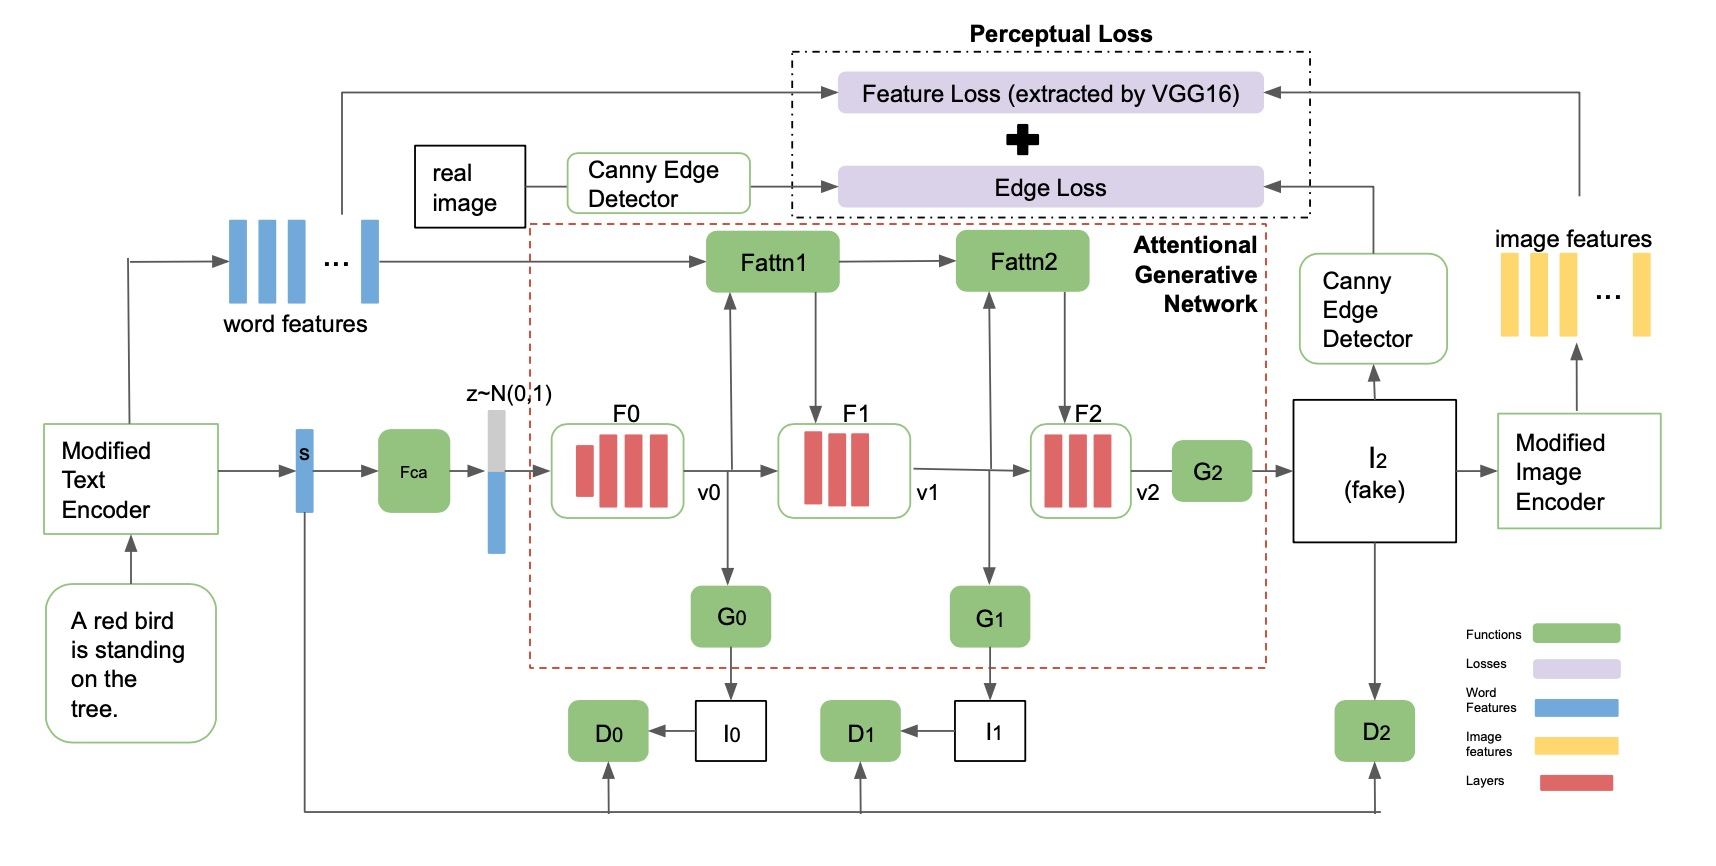
\includegraphics[width=6.5in,height=8.5cm]{1.jpeg}
  \caption{The architecture of our model. Given a sentence S, this text encoder encodes S to a sentence feature vector s as well as a word feature matrix w. We then feed the sentence feature vector and word feature matrix into the network. As shown above, the network has 3 generators which take the hidden visual features v as inputs and generate images I at each stage.}
  \label{ach}
\end{figure*}

\\\\
\noindent The contribution of our work can be addressed in the following two aspects:
\begin{description}
  \item[$\bullet$] Better exploit the text information by modifying the text encoder with the use of pre-trained language models
  \item[$\bullet$] Enforce model to pay attention to the edge by introducing additional constraint on perceptual loss
\end{description}
The above has accelerated the training process of ControlGAN \cite{li2019controllable} and achieved higher Inception Score \cite{salimans2016improved} at the same epoch.

\section{Related Work}
\subsection{Multi-stage generative adversarial networks}
\\\\
\noindent Multi-stage generative adversarial networks have become a commonly adopted architecture when building generative adversarial networks. Zhang et al. proposed a two-stage generative adversarial network architecture (StackGan++)  \cite{zhang2018stackgan++} to generate high-resolution images: Stage-I GAN generates low-resolution images with primitive shapes and colors given textual description, and Stage-II GAN processes the results from the previous stage and text description to yield fine realistic images.
\\\\
Huang et al. \cite{xu2018attngan} proposed an Attentional Generative Adversarial Network (AttnGAN) to allow attention-driven, multi-stage refinement for fine-grained text-to-image generations which focus on drawing the sub-regional details driven by the most relevant words. Li et al. \cite{li2019controllable} also adopted this multi-stage architecture and built a controllable text-to-image generative adversarial network (ControlGAN) which synthesize realistic images through a word-level spatial, channel-wise attention-driven generator that distinguishes visual features. Based on the previous works, we can see that generating images in multi steps from rough to fine is a main trend and a widely used backbone for developing GANs. 



\\
\subsection{Image-Text embeddings}
\\\\
\noindent Well-developed encoders are necessary during texts/images processing. In 2016, Wang et al. proposed a structure-preserving embedding method \cite{wang2016learning} by learning joint embeddings of images and texts using a two-branch neural network with multiple layers of linear projections. This model achieved high accuracy during image-to-text or text-to-image retrievals.
\\\\
The Deep Attentional Multimodal Similarity Model (DAMSM) \cite{xu2018attngan} also provides an image-text matching mechanism by measuring the similarity scores and reducing the mismatch losses of images and texts that are encoded by a CNN net and a LSTM net respectively. Li et al. \cite{li2019controllable} later on remodeled the image encoder by replacing the previous $mix\_6e$ layer of Inception-v3 net with a $relu2\_2$ layer of VGG-16 net. We noticed that a better encoding model can probably be achieved by integrating different embedding models and modifying the objective function to include more detailed losses.\\ 


\section{Proposed Model}
\\\\
\noindent We adopted the proposed model of the channel-wise attention GAN as the main architecture, and explored 2 alternatives as an attempt for improving model performance: in the first approach, we modified the text encoder to make better use of text information. In the second approach, we captured other detailed losses (i.e., edge-loss), and added it to the objective function with a weight of 10*(-3).     
\\\\
In generally, for each given sentence S, our goal is to generate a realistic image I that semantically matches the given text. As shown in the Fig.\ref{ach}, our model has two main components: 1) an Attentional Generative Network that captures latent visual attributes and emphasizes the most relevant subregions during generation. 2) an edge-preserving perceptual reconstruction that aligns item edges of the generated image with the original image. 
\\\\
The attentional generative network takes in the sentence feature vector s and word feature matrix w into the network which contains 3 generators and generates images I at each stage. Specifically, \\
\begin{center}
    $v_0 = F_0(z,Fca(s))$\\
    $v_k = F_k(v_{k-1}, Fattn_k(w, v_{k-1})), k = 1,2$\\
    $I_k = G_k(v_k), k = 0,1,2$.
\end{center}
\\\\
To address our ideas of modification, we conducted the following alternative approaches to modify the text encoder and the objective function: 

\subsection{Approach 1: Make better use of text information by modifying the text encoder}
\noindent One of the main approaches to improve the text-to-image generation is to make better use of text information. In the work of controlGAN \cite{li2019controllable}, the author adopted a bidirectional RNN \cite{xu2018attngan} as text encoder to encode the sentence query. The encoder takes a sentence as input, and outputs two things: 1) a sentence feature s to represent the whole sentence, and 2) a word feature matrix that contains more detailed text information. To improve this existing encoder, we further trained the text encoder with pre-trained word embedding models, as well as adopted Part of Speech(POS) tagging to remove meaningless words in the text.

\subsubsection{Train text encoder based on pre-trained word embedding model}
Using pre-trained language embedding models is one of the most exciting directions in natural language processing (NLP), and is also an exploration of transfer learning. There are many state-of-the-models, such as BERT, RoBERTa, XLNet, and T5. These models, though differ in design, share the same idea of leveraging a large amount of unlabeled text to build a general model of language understanding before being fine-tuned on specific NLP tasks such as sentiment analysis and question answering.
\\\\
In this project, we have experimented with pre-trained  models including GloVe and BERT, to initialize the word embedding of the RNN text encoder model. GloVe(Global Vectors for Word Representation) \cite{pennington2014glove} is a popular embedding technique, trained on aggregated global word-word co-occurrence from a corpus. BERT(Bi-directional Encoder Representations from Transformers) \cite{devlin2018bert} is a even more successful model, which is able to single-handedly achieve state-of-the-art performances on several NLP tasks. 
%The ‘Masked LM’ task is implemented by masking 15% of the word randomly in every sentence and training the model to predict them. The ‘SOP’ task is a classification task with two sentences input and the model is expected to recognize the original order between these 2 sentences, which increases it’s document level understanding. The impact these training tasks create and the internal working of BERT requires a more detailed analysis which I will not go into right now.

\subsection{Approach 2: Add additional constraints by including external losses}
\noindent External losses, such as box loss, pixel loss, image adversarial loss etc., are regraded as efficient methods for improving the performance of GANs. 

\subsubsection{Feature Loss extracted by VGG16}
 To mitigate the randomness of the generated images, perceptual loss calculation is an important approach to quantize the fidelity of the generated images. While pixel-wise difference is sensitive to the colors, a way of measuring distance between generated images and ground truth images is to apply metric learning. ControlGAN \cite{li2019controllable} backpropogated the mean square error (MSE) between visual features of real images and fakes images outputted from a relu layer of VGG16 as its perceptual losses.
 Measuring perceptual losses of real and fakes images mainly captures the visual feature disparities, and thus performs well when being included in the objective function.  
 
 \subsubsection{Edge Loss captured by canny edge detector}
 We noticed that a big amount of generated images, through semantically align with the text query, are visually out of shape. As shown in the figure \ref{niao}, this generated image obviously contains bird-related features like feathers and beaks, but lacks an acceptable shape of bird. 

\begin{figure}[htp]
    \centering
    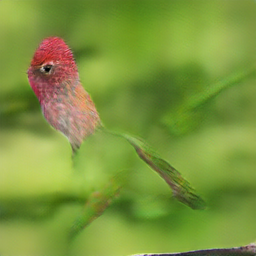
\includegraphics[width=0.56\columnwidth]{bd1.png}
    \caption{A generated bird with bird features but in a bad shape }
    \label{niao}
\end{figure}

\noindent In our attempt, we conducted an edge-preserving perpetual loss calculation that takes edge information of the real and fake images to generate images with meaningful shapes. For each image generated by G2 (the generator in the final stage), we extracted edge information by applying a canny edge detection algorithm to this fake image and its corresponding real image. 
\\\\
The canny edge detection process removes noise in the image with a 5x5 Gaussian filter, and then filters the image horizontally and vertically with a Sobel operator to get the pixel gradients in both directions. After getting gradient magnitudes, edges are detected at which the pixel gradients change dramatically. For each image, this algorithm removes those unwanted pixels which don’t contribute to edge formation, generating a new grayscale edge map that contains only the item edges. 


\subsubsection{Image-Text Embedding}
To extract the edge image embedding, we adopted a deep structure-preserving image-text embedding approach \cite{wang2016learning}. This method is able to learn joint embeddings of images and text using a two-branch neural network. That’s to say, the image and the text will share a latent space where vectors from the two modalities can be compared directly. Though in our task, we don’t need to measure the semantic similarity between visual data and text data, but we need to measure the similarity of the edge from the generated image and the real image. We could utilize this method because in the learned latent space, images with similar meaning would be close to each other. Therefore, after training the two-branch model(Fig.\ref{embeddingmodel}), we selected the image sub-network to encode the edge images to the target embeddings. Based on this, we could be able to calculate the edge loss that we proposed. 
\\\\
\begin{figure*}[htp]
    \centering
    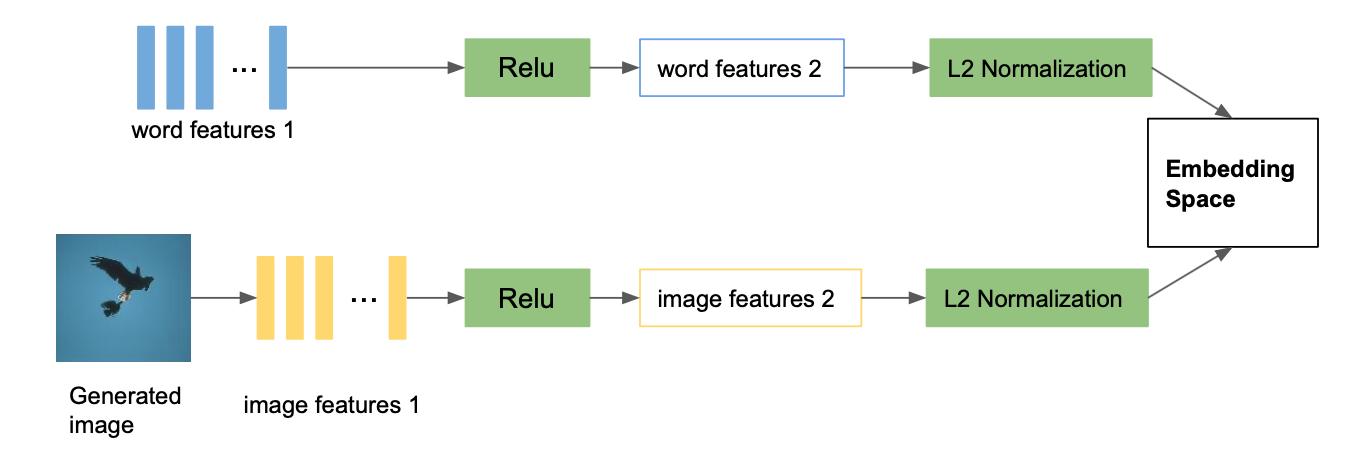
\includegraphics[width=0.75\textwidth]{ebd.png}
    \caption{Model structure: there are two branches in the network, one for images ($X$) and the other for text ($Y$). Each branch consists of fully connected layers with ReLU nonlinearities between them, followed by L2 normalization at the end \cite{wang2016learning}.}
    \label{embeddingmodel}
\end{figure*}

\noindent \textbf{Model Architecture.} The model architecture is in Fig.\ref{embeddingmodel}. As shown in Fig.\ref{embeddingmodel}, our model has two branches, each composes of fully connected layers with weight matrices $W_l$ and $V_1$ . Two linear layers are separated by a ReLU activation function. After the last fully connected layer, we applied L2 batch normalization.
\\\\
\textbf{Training Objective.}  Our training objective is a stochastic margin-based loss that includes bidirectional cross-view ranking constraints. Given a training image $x_i$ , let $Y_i^+$ and $Y_i^-$ denote its sets of matching (positive) and non-matching (negative) texts, respectively. We want the distance between $x_i$ and each positive text $y_j$ to be smaller than the distance between $x_i$ and each negative text $y_k$ by some enforced margin $m$: 
\begin{center}
    $d(x_i,y_i) + m < d(x_i,y_k) \quad {\forall}y_j \in Y_i^+, {\forall}y_k \in Y_i^-. $
\end{center}
Similarly, given a text $y_{i^'}$, we have
\begin{center}
    $d({x_{j^'}},{y_{i^'}}) + m < d({x_{k^'}} , {y_{i^'}}) \quad {\forall}{x_{j^'}}\in {X_{i^'}}^+, {\forall}{x_{k^'}} \in {X_{i^'}}^-. $
\end{center}
\\\\
\textbf{Loss Functions.}  We converted the constraints to our training objective in the standard way using hinge loss. The resulting loss function is given by 
\begin{center}
    $$L(X,Y) = \sum_{i,j,k}max[0, m + d(x_i,y_i) - d(x_i, y_k)] + \\  \quad  \quad \sum_{i,j,k}max[0, m + d({x_{j^'}},{y_{i^'}}) - d({x_{k^'}},{y_{i^'}})]$$
\end{center}
\\\\
\textbf{Triplet Sampling.}  Our loss involves all triplets consisting of an anchor input, a positive match of the same class as the anchor, and a negative match of a different class from the anchor. To improve the optimizing efficiency, we sampled triplets within each mini-batch and optimized our loss function using SGD. As the Fig.\ref{triplet} shows, the triplet loss minimizes the distance between an anchor and a positive, both of which have the same identity, and maximizes the distance between the anchor and a negative of a different identity.
\begin{figure}
    \centering
    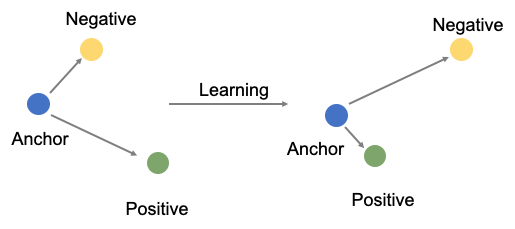
\includegraphics[width=0.95\columnwidth]{fig/tripletloss.png}
    \caption{The Triplet Loss minimizes the distance between an anchor and a positive, both of which have the same identity, and maximizes the distance between the anchor and a negative of a different identity}
    \label{triplet}
\end{figure}
\\\\
\textbf{Features and Network Settings.} To train the Image-Text Embedding network, we extracted edge information by applying a canny edge detection algorithm to CUB dataset. The canny edge detection process removes noise in the image with a Gaussian filter, and then filters the image horizontally and vertically, generating a new edge map that contains only the item edges. We removed color messages from the captions and applied BERT to encode text. The encoded text features and edge features are parsed into the network. The adversarial learning enforces edge features and text features to lean toward the same feature vector. Image embedding model takes 256*256 image and maps it to a 300-dimension feature vector, while text embedding model parses a sentence feature with dimension 300.
\\\\
\textbf{Application in perceptual loss.} Besides the feature difference obtained from the pre trained VGG-16 network, we included the edge loss when computing perceptual loss. We connected the image embedding model that trained separately to the stage of perceptual loss, and parsed the edge  into the image embedding network. A new perceptual loss is defined as:
\begin{center}
    $L\_percep(I,{I^'}) = L\_feature(I,{I^'}) + 10^{-3}* L(edge) $
\end{center}

\section{Evaluation}
\subsection{Datasets}
Our work is evaluated on CUB bird  \cite{WelinderEtal2010}, consisting of 8,855 training images, 2,933 test images, and 10 corresponding captions per image. 

\subsection{Implementation}
We maintained the training setup of the original work which used Adam optimiser with the learning rate 0.0002. To evaluate the enhanced text encoders with pre-trained models including BERT and GloVe, we changed the text-encoders and image-encoders (co-trained with the text-encoder), while keep other settings the same. To study the impact of edge loss, we adopted its own text-encoder and image-encoder, and solely modified the layer of perceptual loss.  

\section{Ablation Studies}
\noindent The original model was trained for 600 epochs. In order to assess the effectiveness of our work, we extracted the output from the 15th epoch of each model and used the Inception Score(IS) \cite{salimans2016improved} of generated testing images. According to quantitative results shown in Table.1, our approaches achieved higher Inception Scores at the 15th epoch, indicating that the proposed changes on the model can effectively promote the training process at early stage. In addition, we presented a visual comparison(Fig.\ref{sample}) of the generated images from different model settings given the same caption. 
\\\\

\begin{table}[htp]
    \centering
    \begin{tabular}{lll}
    \toprule
      \textbf{Model}   &\textbf{IS Mean }  & \textbf{IS Std}\\
      \midrule
      ControlGAN \cite{li2019controllable}   &2.9145 & 0.0600\\
      \midrule
      Ours\_Bert & 3.9473 & 0.4371 \\ 
      \midrule
      Ours\_GloVe & 4.5177& 0.2305 \\ 
      \midrule
      Ours\_EdgeLoss & 3.8083 & 0.3646 \\
      \bottomrule
    \end{tabular}
    \label{test}
    \vspace{3mm}
    \caption{The test results extracted from  the  15th  epoch  of  each  model. To evaluate the enhanced text encoders, we changed the text-encoders and image-encoders (co-trained with the text-encoder), while kept other  settings  the  same. To study the impact of edge loss, we adopted its own text-encoder and image-encoder, and solely modified the layer of perceptual loss }
    
\end{table}
\begin{figure}[htp]
    \centering
    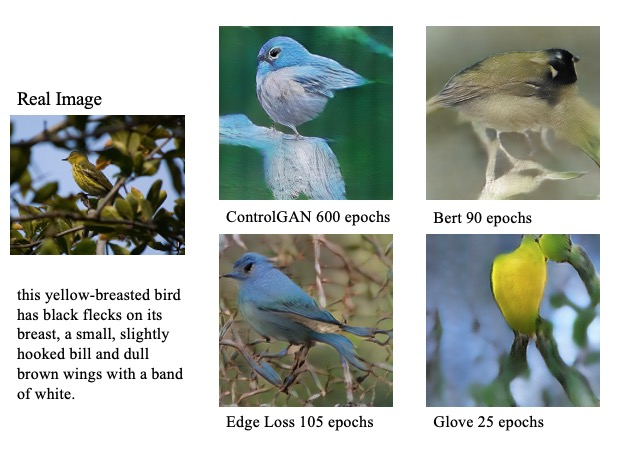
\includegraphics[width=0.95\columnwidth]{fig/samples.jpeg}
    \caption{The generated samples}
    \label{sample}
\end{figure}
\noindent \textbf{Effectiveness of advanced text-encoder.} The models using enhanced text encoder with pre-trained model BERT and GloVe are able to generate yellow breast even with a smaller amount of training epochs. Since the model with edge loss utilizes the same text encoder as the ControlGAN, they both generated a blue bird. Adopting an advanced text-encoder can better capture semantic details and contribute to rendering correct colors to the image.
\\\\
\noindent \textbf{Effectiveness of additional edge loss.} The model with edge loss seems to have a clearer shape of bird and a rich background than the others.
\\\\
\section{Conclusion}
Based on ControlGAN\cite{li2019controllable}, we proposed better text encoders to utilize the text information and enforced the model to pay attention to the edge by introducing additional constraint on perceptual loss. We effectively achieved  higher  Inception  Score at the same epoch comparing against the original ControlGAN\cite{li2019controllable}, which demonstrated the advantages of our method with respect both to high quality image-generation and efficiency of learning. 

{\small
\bibliographystyle{ieee}
\bibliography{egbib}
}

\end{document}



